%%%%%% /!\ AUTHOR : Guillaume Van Dessel || DATE : 19.10.2015 
\chapter{Ondes mécaniques et acoustiques} 

Ce troisième chapitre est consacré aux ondes dites \textit{\textbf{mécaniques}}. Nous verrons ainsi toutes les analogies entre ondes EM et ondes mécaniques ainsi que certaines différences qui subsistent entre ces deux types d'onde. \\ 

Il est important de mentionner que les ondes EM se propagent sans l'aide d'un \textit{support matériel}, c'est là leur grande différence en comparaison avec les ondes mécaniques, qui ont besoin de "matière" pour qu'il y ait propagation. 

\section{Ondes mécaniques : Exemple de la corde vibrante}

Admettons qu'il existe une corde \textit{parfaitement souple et élastique}\footnote{Pas de couple de torsion.} dans un référentiel exempt de \textit{potentiel gravitationnel} \footnote{Ou alors dont l'effet de la pesanteur est \textit{\textbf{négligeable.}}}. La \textit{tension} longitudinale $F$ le long de la corde est supposée \textit{constante} et les déplacements longitudinaux sont considérés comme \textit{\textbf{négligeables}}. \\Seuls les déplacements verticaux sont pris en compte et nous noterons : $\vec{\xi}(x,t) = y(x,t) \vec{a}_{y}$.
\\
Nous admettrons aussi que lorsqu'une déformation se déplace le long de la corde, le reste de la corde n'est pas visé par la déformation et se trouve dès lors au \textit{repos} en ce sens où chacun des points du reste de la corde présente un déplacement vertical nul : $\vec{\xi}(x_{r},t) = \vec{0}$. \\

Considérons alors un déplacement vertical sur une portion de corde $\Delta x$ comme représenté sur la figure ci-après.  La pente de la corde dans le plan XY lorsque $\Delta x$ tend vers $0$ est donnée par $\tan (\alpha) = \frac{\partial y}{\partial x}$.

\begin{center}
	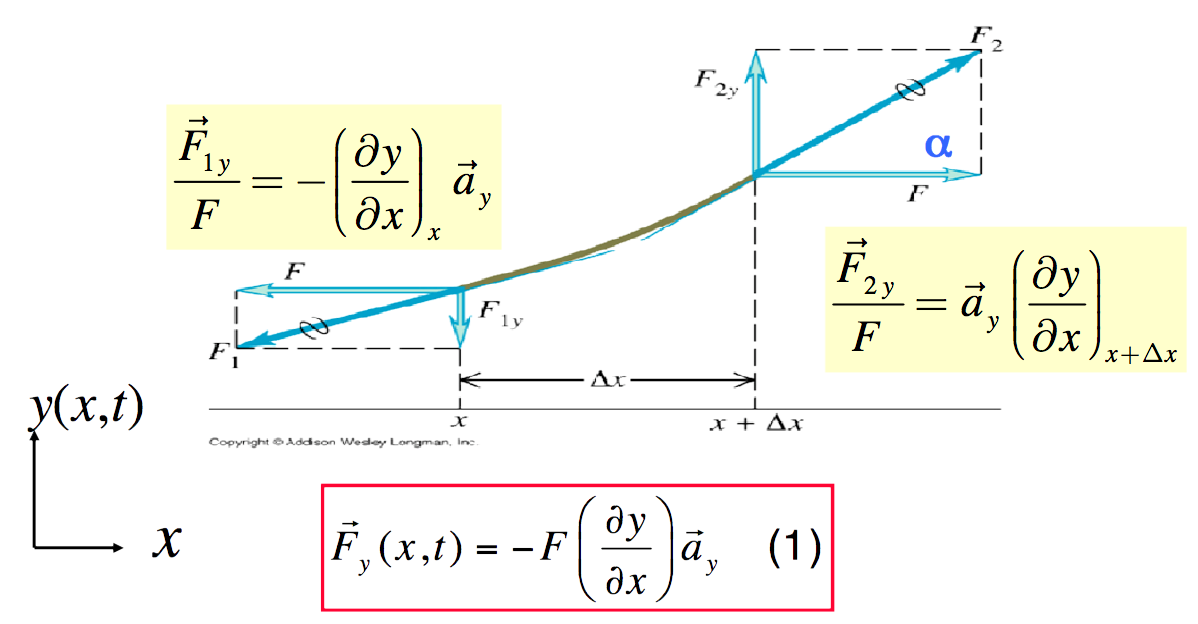
\includegraphics[width = 0.8\linewidth]{SlideCM3.png}
\end{center}

Les forces verticales en $x$ et $x+\Delta x$ valent respectivement

\begin{equation}
\vec{F}_{1y}(x,t) = - F  (\frac{\partial y}{\partial x})|_{x}  \vec{a}_{y} 
\label{Force1}
\end{equation}

\begin{equation}
\vec{F}_{2y}(x+\Delta x,t) = F (\frac{\partial y}{\partial x})|_{x+\Delta x} \vec{a}_{y}
\label{Force2}
\end{equation}

Si nous dérivons par rapport au temps, nous obtenons (en écrivant désormais $\vec{F}_{1y} = \vec{F}_{y}(x)$, puisqu'on fait tendre $\Delta x$ vers $0$, et donc qu'on s'intéresse à la force en $x$),

\begin{equation}
\frac{\partial \vec{F}_{y}}{\partial t} = - F (\frac{\partial^{2} y}{\partial t \partial x}) \vec{a}_{y}
\label{Force3}
\end{equation}

\begin{equation}
\frac{\partial \vec{F}_{y}}{\partial t} = - F (\frac{\partial u}{\partial x}) \vec{a}_{y}
\label{Force4}
\end{equation}

où $u$ est la norme de $\vec{u}(x,t)$ qui est \textbf{la vitesse verticale de déplacement d'un point de masse de la corde en fonction de sa position longitudinale $x$ et du temps $t$}. \\ 

Si nous dérivons désormais par rapport à $x$, nous obtenons une nouvelle identité intéressante : 

\begin{equation}
\frac{\partial \vec{F}_{y}}{\partial x} = -F \frac{\partial^{2} y}{\partial x^{2}} \vec{a}_{y} 
\label{ForceLOL}
\end{equation}

Etablissons un bilan des forces dans la direction verticale : 

\[\sum_{i} \vec{F}_{y} = \vec{F}_{1y} + \vec{F}_{2y}  = F [\frac{\partial y}{\partial x}|_{x+\Delta x} - \frac{\partial y}{\partial x}|_{x}] \vec{a}_{y} \]

Etant donné que $\Delta x$ est supposé tendre vers $0$, en multipliant par $\Delta x$ en haut et en bas de la fraction : 

\begin{equation}
\sum \vec{F}_{y} \Rightarrow \lim_{\Delta x \to 0}  F \Delta x \frac{[\frac{\partial y}{\partial x}|_{x+\Delta x} - \frac{\partial y}{\partial x}|_{x}]}{\Delta x} \vec{a}_{y} = F \Delta x \frac{\partial^{2} y }{\partial x^{2}} \vec{a}_{y} 
\label{Force5}
\end{equation}

Par la troisième \textit{loi de \textbf{Newton}}, nous égalons l'expression trouvée au produit d'une masse par une accélération (donnée par la dérivée de la vitesse):
\begin{equation}
\sum \vec{F}_{y}  = m \frac{\partial^{2} y }{\partial t^{2}} \vec{a}_{y} =  (\mu \Delta x) \frac{\partial u }{\partial t} \vec{a}_{y}  
\label{Force6}
\end{equation}
où $\mu$ est la masse linéique de la corde (masse par unité de longueur).

Nous pouvons dès lors mettre en exergue la relation liant l'équation \eqref{Force5} et l'équation \eqref{Force6} : 

\begin{equation}
\frac{\partial^{2} y }{\partial t^{2}} = \frac{F}{\mu}  \frac{\partial^{2} y }{\partial x^{2}}
\label{EqOnde}
\end{equation}

ce qui représente exactement le même type d'équation que nous avons abordé à la section précédente! 
En effet, le scalaire $\sqrt{\frac{F}{\mu}}$ équivaut ici à la vitesse de propagation de l'onde.  \\
De même, nous observons que nous retrouvons des \textbf{EDP couplées} en $F_{y}$ et $u$. \\
Afin de s'en convaincre, nous utilisons les équations \eqref{Force4}, \eqref{ForceLOL} et \eqref{EqOnde} :

\[ \frac{\partial F_{y}}{\partial t} = - F (\frac{\partial u}{\partial x})\]

\[ \frac{\partial F_{y}}{\partial x} = -F \frac{\partial^{2} y}{\partial x^{2}} = -\mu \frac{\partial^{2} y}{\partial t^{2}} = -\mu \frac{\partial u}{\partial t} \]

La résolution de l'équation \eqref{EqOnde} s'établit de la même manière que pour les ondes EM. \\ 
Bien entendu, les deux grandeurs scalaires impliquées dans les équations couplées admettent cette même propriété
d'\textit{impédance caractéristique}. En effet, étant donnée leur caractéristique physique, il convient que le paramètre $\mathcal{K}$ 
dans $F_{y}(x,t) = \mathcal{Z}u(x,t) + \mathcal{K}$ soit \textit{nul}. \\ 
Nous avons alors, 

\[\frac{F_{y}(x,t)}{u(x,t)} = \mathcal{Z} = \sqrt{F\mu} \hspace{8pt} [N\cdot s / m]\]

Étant donné que la corde se déplace sous l'effet d'une force, nous pouvons conclure que $\vec{F_{y}}$ exerce un travail sur la corde. 
La puissance étant par définition un travail par unité de temps, nous avons que le produit scalaire entre la force et la vitesse de son point d'application 
donne la puissance recherchée en un temps et un point donné sur l'axe :
\[P(x,t) = \vec{F}_{y}(x,t) \cdot \vec{u}(x,t) \]
Comme $\vec{F}_{y}$ et $\vec{u}$ ont la même direction, nous écrirons alors dans ce cas : 
\[ P(x,t) = F_{y}(x,t) u(x,t) = \mathcal{Z} u^{2}(x,t) = \sqrt{F \mu}\: u^{2}(x,t) = \frac{F_{y}^2(x,t)}{\mathcal{Z}}\]
Si nous considérons que le signal de l'onde mécanique le long de la corde est de \textit{type sinusoïdal}, 
nous pouvons entreprendre de calculer la valeur moyenne (sur une période) de la puissance de l'onde. 

Soit donc $\vec{y}(x,t) = \xi_{0} \cos(kx-\omega t) \vec{y}$ et dès lors $\vec{u}(x,t) = \omega \xi_{0} \sin(kx-\omega t) \vec{y}$, la \textit{valeur moyenne de ce signal \textbf{au carré}} sur un nombre entier de périodes vaut $\frac{\xi_{0}}{2}$, dès lors : 
\[ \overline{P(x,t)} = \frac{\mathcal{Z} u^{2}_{max}}{2} = \frac{\omega^{2} \xi_{0}^{2}}{2} \mathcal{Z}\]
Nous pouvons aussi définir des concepts comme celui d'\textit{énergie cinétique} de la corde en un \textit{tronçon infinitésimal} et un temps donnés. \\
Cette énergie cinétique vaut le produit de la masse de ce très petit tronçon, considéré comme un point de masse équivalente au tronçon, et du carré de sa vitesse
verticale en $t$. 
\[\Delta U_{k}(x,t) = \frac{(\mu \Delta x)u^{2}(x,t)}{2} \] 
La valeur maximale de cette expression (par unité de longueur) se donne par la relation : 
\[U_{k,max} = \frac{\mu u_{max}^{2}}{2}\]
Nous définissons encore le concept d'énergie \textit{potentielle de déformation} comme l'énergie du couple de forces $\vec{F}_{1y}$ et $\vec{F}_{2y}$, obtenue en multipliant la force verticale par la variation de l'angle $\alpha$
\[\Delta W = (F_{y}(x,t) \Delta l)(-\Delta \alpha)= F_{y}(x,t) \Delta l \frac{\Delta F_{y}(x,t)}{F} \]
\[\hspace{2cm} \Delta W = \frac{\Delta l}{F} \int_{0}^{F_{y}(x,t)} F_{y'} dF_{y'} = \frac{F_{y}^{2}(x,t)}{2F}\Delta l \]

Encore une fois, la valeur maximale de cette expression (par unité de longueur) s'écrit : 

\[U_{p,max} = \frac{F_{y,max}^{2}}{2F}\]

Nous remarquons alors que ces deux valeurs sont \textit{équivalentes}! 
\\ En effet, comme $F_{y}^{2}(x,t)  = \mathcal{Z}^{2} u^{2}(x,t)$, nous pouvons écrire 

\[ U_{k,max} = \frac{\mu u_{max}^{2}}{2} =   \frac{\mathcal{Z}^{2} u_{max}^{2}}{2F} = \frac{F_{y,max}^{2}}{2F} = U_{p,max}\]

A titre de complément\footnote{Image tirée de l'adresse suivante : \url{https://ccrma.stanford.edu/realsimple/lab_inst/img31.png}}, voici la \textit{distribution de l'énergie d'une corde vibrante soumise à un \textbf{amortissement de son amplitude}} (le \textit{frottement }dissipant de l'énergie en chaleur peut être une cause de l'atténuation) : 
\begin{center}
	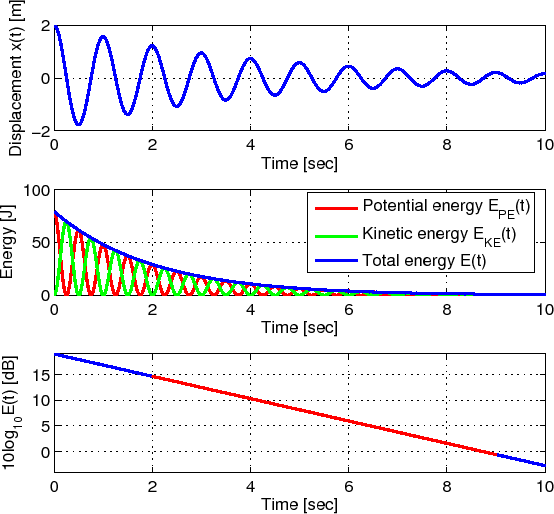
\includegraphics[width = \linewidth]{BIG.png}
\end{center}



\section{Ondes acoustiques}

Etant donnée la complexité apparente du phénomène en 3D, nous allons aborder ici le cas simplifié et \textit{\textbf{moins général}} d'une 
\textit{onde acoustique} 1D. A nouveau, nous parlons ici d'une onde \textit{\textbf{mécanique}}, c'est à dire qu'elle nécessite un support physique afin 
de pouvoir se propager dans l'espace. Cependant, nous la distinguons du cas de la corde vibrante de la section précédente à ce point-ci près; 
elle est non plus \textit{transversale}, mais bien \textit{\textbf{longitudinale}}. Les déformations du milieu traversé par l'onde ne sont plus perpendiculaires mais 
bien dans le sens du
\textit{déplacement}
de l'onde.

\subsection{Hypothèses}

Afin de pouvoir écrire les équations qui vont suivre sereinement, il nous faut dresser une liste d'hypothèses qui justifieront les écritures. 
Tout d'abord, il faudra admettre que nous travaillons avec un milieu (\textit{par exemple ici de l'air}) aux propriétés thermodynamiques \textit{parfaites}. \footnote{Source : \url{https://fr.wikiversity.org/wiki/Introduction_à_l\%27acoustique/Équation_d\%27onde}}
Nous considérons les déplacements longitudinaux comme respectant la condition $L = \sqrt{DT} << \lambda^{2}$ où $\lambda^{2}$ est le carré de la longueur d'onde, $D$ le coefficient de diffusion de l'onde et 
$T$ une période de l'onde. Ceci implique l'isentropie et l'absence de phénomènes thermodynamiques irréversibles dont l'effet sur les équations est difficilement abordable dans le cadre de ce cours. \footnote{Pour plus de formalisme, se référer à \url{https://fr.wikiversity.org/wiki/Introduction_à_l\%27acoustique/Hypothèse_acoustique}} \\ 
Une fois tout ceci dit, nous pouvons posément commencer. Nous allons nous attarder sur le cas d'une propagation dans l'air et, sans le démontrer, accepter que ce raisonnement tienne pour la propagation dans 
d'autres milieux.

\subsection{Équations constitutives} 

Nous considérons le mouvement (en avant et en arrière) des particules  lors de la compression et de la dilatation (réversible) d'un gaz parfait dans un cylindre de section $A$. On note par $p_{y}$ la pression différentielle $\Delta p$ par rapport à la pression au repos.\\

\textbf{Loi de \textit{Newton}} : Sous forme \textit{scalaire} car la direction de déplacement des particules est supposée tout le temps horizontale et en phase avec le déplacement
de droite à gauche du piston, la loi de Newton nous fournit une relation entre la force exercée sur le gaz par le piston (la pression "\textit{locale}" aux points d'application, en notant que la pression est une force par unité de surface) et la dérivée de la vitesse des particules à ces endroits. \\ 

Nous écrirons ceci : 

$$F_{y} = -p_{y} A = m \frac{\partial{u}}{\partial t}$$ 

En notant qu'une tranche d'air d'épaisseur $\Delta x$  au repos occupe un volume $A\Delta x$, et en multipliant chaque terme par $\Delta x$, nous obtenons 
$$-p_{y} A\Delta x = \Delta x m \frac{\partial{u}}{\partial t}$$ 

Passant à  un volume \textit{infinitésimal} et définissant la masse volumique 
$\rho_{0}$ comme la masse par unité de volume, la loi de Newton se ramène à

\[\frac{\partial p_{y}}{\partial x} = - \rho_{0} \frac{\partial{u}}{\partial t}\]


\textbf{Loi de la conservation de la masse}  : Elle nous indique que si le volume diminue, la pression augmente, en vertu de la définition du module d'élasticité isostatique $B$, qui relie la pression à la variation relative de volume:
\[\Delta p  = - B \frac{\Delta V}{V} \]

Dans notre cas, $\Delta p = p_y$, $V = A \Delta x$ et $\delta V = A \Delta y$, puisque $\Delta y$ est la variation de largeur de la tranche d'air sous l'effet de la pression $p_y$. On obtient donc, en passant à la limite:

\[p_{y}  = - B \frac{\partial y}{\partial x}\] et en dérivant par rapport au temps,

\[\frac{\partial p_{y}}{\partial t} =  - B \frac{\partial u}{\partial x}\]


Une fois de plus, nous avons affaire à des EDP linéaires couplées du premier ordre. Il en résulte que les grandeurs physiques \textit{force} ou \textit{pression} (selon que l'on multiplie par $A$ ou non) et 
\textit{vitesse longitudinale} sont liées et vérifient l'équation d'onde. La vitesse de propagation du signal vaut donc machinalement : $v = \sqrt{\frac{B}{\rho_{0}}}$\footnote{Si nous considérons la vitesse du son à travers un solide : $v = \sqrt{\frac{Y}{\rho_{0}}}$ où $Y$ est le module de \textit{Young}.}.  Si nous travaillons bien avec des
gaz \textbf{parfaits}, nous pouvons écrire : $$p_{0} = \frac{nRT}{V_{0}}= \frac{mR^{*}T}{V_{0}} = \rho_{0}R^{*}T \Rightarrow v = \sqrt{\frac{\gamma RT}{M}}$$ où $M$ est la \textit{masse molaire} du gaz. \\
Prenons le cas de l'air, $\gamma$ est considéré comme une constante (voir \textit{Transformations adiabatiques réversibles}) et vaut approximativement $1.4$, $M$ quant à elle
vaut à peu près $0.02896 [kg/mol]$. Nous avons alors une expression approchée de la \textit{vitesse du son dans l'air} à température $T$. 

\[ v \simeq \sqrt{\frac{\gamma R}{M}} \sqrt{T} \simeq 20.05 \sqrt{T} \Rightarrow \hspace{5 pt} \mbox{pour $T = 293.15[K]$ : } \hspace{5pt} v \simeq 343.3 [m/s]\]

\subsection{Puissance et intensité}

De manière analogue\footnote{Selon les unités, le cas de la \textit{corde vibrante} renseignait sur la puissance et \textbf{non} l'intensité} aux autres cas d'ondes mécaniques, nous pouvons définir l'intensité d'une onde acoustique comme le produit de son \textit{impédance caractéristique}
par la norme de la \textit{vitesse} de la déformation locale du milieu. \\ 
Nous avons alors, 

\[I(x,t) = \mathcal{Z} u^{2}(x,t) = \frac{p_{y}^{2}(x,t)}{\mathcal{Z}}\]

dans un cas \textit{sinusoïdal}%\footnote{ C'est à dire où $y(x,t) = \xi_{max} cos(kx-\omega t)$} 
, nous pouvons définir également une intensité \textit{moyenne} sur une période : 

\[ |I_{moy}| = \frac{\mathcal{Z} u^{2}_{max}}{2} = \frac{\sqrt{B \rho_{0}} \omega^{2} \xi_{max}^{2}}{2}\]

Notons que $\mathcal{Z}$ dépend de facteurs thermodynamiques comme la température, c'est pourquoi nous pouvons écrire aussi sous une autre forme l'intensité moyenne en fonction de
la pression maximale locale : 

\[ |I_{moy}| = \frac{p_{max}^{2}}{2 \mathcal{Z}} \Rightarrow \hspace{5pt} \mbox{pour $T = 293.15[K]$ , 2 $\mathcal{Z} \simeq 825.6$  : } \hspace{5pt} I_{moy} = \frac{p_{max}^{2}}{825.6}\]

\begin{center}
	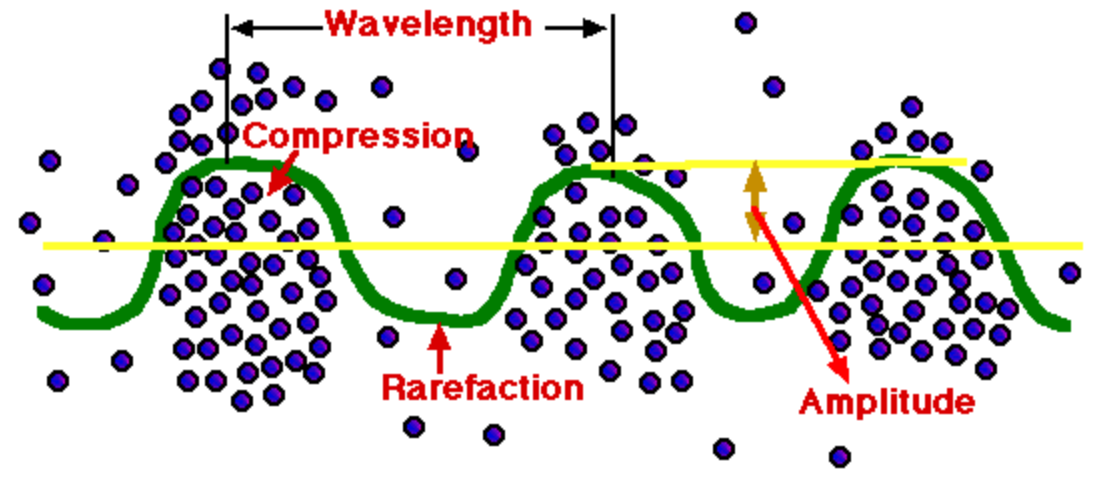
\includegraphics[width = 0.9\linewidth]{pression.png}
\end{center}

\section{Ondes planes, cylindriques et sphériques}

Nous avons introduit le \textbf{vecteur de \textit{Poynting}} à la fin de la section concernant les ondes EM. La puissance totale d'une source \textit{ponctuelle} se donne par l'expression 

\[P_{tot} = \oint \vec{S} \cdot d\vec{A}\]

Dans le cas de propagations symétriques dans des configurations spéciales, nous pouvons déduire l'expression des champs électriques et magnétiques et leur \textit{décroissance} apparente, comme 
lorsque nous jetons une pierre dans une mare et voyons la propagation de type circulaire autour de la singularité. 

\subsection{Ondes sphériques} 

L'intensité perçue à une distance $r = \sqrt{x^{2} + y^{2} + z^{2}}$ de la source est proportionnelle à $\frac{1}{r^{2}}$ car la relation impliquant le vecteur de Poynting nous 
donne $P_{tot} = 4 \pi r^{2} I$. \\ 
Comme nous savons que l'intensité d'une onde EM est proportionnelle à la norme du vecteur de Poynting (de par sa définition même!), nous pouvons écrire 

\[ EH \propto \frac{1}{r^{2}} \Rightarrow E,H \propto \frac{1}{r}\]

Nous avons de manière générale, en admettant un terme \textit{d'Alembert} homogène, une expression du champ électrique : 

\[\vec{E}(\vec{r},t) = \frac{1}{r} \:f(r-vt) \:\hat{u}_{r},\] 

et pour une onde sphérique \textit{monochromatique sinusoïdale},

\[\vec{E}(\vec{r},t) = \frac{E_{0}}{r} \sin(kr-\omega t) \hat{u}_{r} = \frac{E_{0}}{r} \sin(k(r- vt)) \hat{u}_{r}, \]

où $\hat{u}_{r}$ est un vecteur unitaire dont la direction est orthogonale au vecteur de propagation (depuis le centre vers $\vec{r}$).


\subsection{Ondes cylindriques} 

L'intensité perçue à une distance $r = \sqrt{x^{2} + y^{2}}$ de la source est proportionnelle à $\frac{1}{r}$ car la relation impliquant le vecteur de Poynting nous 
donne $P_{tot} = 2 \pi r h I$. \\ En effet, il faut s'imaginer un exemple de source \textbf{non plus ponctuelle} mais \textit{linéique} à l'instar d'un champ magnétique à une 
distance $r$ d'un courant linéique. Chaque source ponctuelle présente sur le "fil" donne lieu à une propagation sphérique mais toutes ces propagations sphériques mises bout à bout donnent 
des \textit{fronts d'onde} sous forme d'enveloppes cylindriques concentriques autour de ce même "fil" de source linéique. Si nous imaginons un "fil" infini, à la limite,
nous avons bien la relation liant la puissance totale à l'enveloppe d'un cylindre de hauteur $h$. Si le fil est fini, cette relation est une approximation tout à fait valable sauf 
aux bords.

Comme nous savons que l'intensité d'une onde EM est proportionnelle à la norme du vecteur de Poynting (de par sa définition même!), nous pouvons écrire 

\[ EH \propto \frac{1}{r} \Rightarrow E,H \propto \frac{1}{\sqrt{r}}\]

Nous avons de manière générale, en admettant un terme \textit{d'Alembert} homogène, une expression du champ électrique : 

\[\vec{E}(\vec{r},t) = \frac{1}{\sqrt{r}} f(r-vt) \hat{u}_{r},\] 

et pour une onde cylindrique \textit{monochromatique sinusoïdale},

\[\vec{E}(\vec{r},t) = \frac{E_{0}}{\sqrt{r}} \sin(kr - \omega t) \hat{u}_{r} = \frac{E_{0}}{\sqrt{r}} \sin(k(r - v t)) \hat{u}_{r}\]

où $\hat{u}_{r}$ est ici un vecteur unitaire dont la direction est orthogonale au vecteur de propagation (depuis la projection orthogonale de $\vec{r}$ sur la source linéique jusqu'à $\vec{r}$ lui-même).


\subsection{Ondes planes} 

Le cas d'une propagation plane tout comme celui d'une propagation cylindrique est "\textit{idéal}" et n'est pas réellement envisageable physiquement. \\
Quoi qu'il en soit, nous pouvons tout de même faire l'expérience d'esprit qu'une onde puisse, pour tous les $\vec{r}$ présents sur un plan dont la normale est la direction 
de propagation, avoir la même intensité pour ses composantes (champ électrique ou magnétique). Nous y reviendrons à la prochaine section. \\

Dans ce cas-là, toute la puissance est \textit{partagée} à chaque fois sur chaque même plan infini (ils sont parallèles entre eux) et nous \textbf{n'observons plus} de décroissance 
en $1/r^{n}$! Nous écrivons alors simplement les relations suivantes : 

\[E,H \propto 1\]

\[\vec{E}(\vec{r},t) = E_{0} \sin(\vec{r}\cdot \vec{k}-\omega t) \hat{u}_{r}\]

où $\hat{u}_{r}$ est un vecteur unitaire dont la direction est orthogonale au vecteur de propagation.

\section{Effet Doppler}

Considérons des référentiels galiléens et \textit{négligeons les effets relativistes}. 
Si la source d'une onde ou bien son observateur se déplacent l'un par rapport à l'autre, l'observateur, malgré une \textit{pulsation identique}, verra les fronts d'onde avec une fréquence différente de celle de la source! \\ 

Nous allons uniquement étudier ce phénomène en régime dit "\textit{stationnaire}" car si la fréquence de la source varie ou que la vitesse de la source varie ou que celle-ci 
passe à proximité directe de l'observateur et le dépasse, l'observateur aura droit à une phase "\textit{transitoire}" qui ne respectera pas à la lettre la loi que nous allons énoncer.  \\

Nous garderons à l'esprit qu'une vitesse \textbf{positive} est une vitesse dans le sens \textit{source $\rightarrow$ observateur}.

L'effet Doppler est décrit par l'équation suivante, à vitesses $v_{o}$ et $v_{s}$ constantes et dans un même milieu de propagation (vitesse de l'onde $v$ constante) : 

\[f_{o} = \frac{v-v_{0}}{v-v_{s}}f_{s}\]

On peut écrire cette relation sous la forme
$$ f_{o} = f_s\Big(1+\frac{v_s-v_{0}}{v-v_{s}}\Big)$$
Dans le cas où $v_{o},v_{s} << v$, le terme $v-v_s$ vaut approximativement $v$ et nous ramenons l'égalité précédente à 

\[f_{o} \simeq f_{s} (1 + \frac{\Delta v_{s,o}}{v}) \]
avec $\Delta v_{s,o}=v_s-v_0$.

\textbf{Notons} toutefois la version \textit{relativiste} de l'effet Doppler, d'application traditionnellement lorsque $v \geq 10^{-1} c$ : 
\[  f_{o} = \sqrt{\frac{c-v}{c + v}} f_{s}\]

\begin{figure*}
	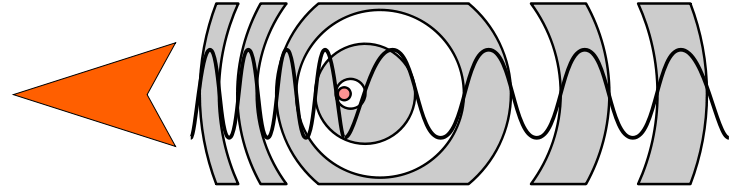
\includegraphics[width = 0.65\linewidth]{doppler.png}
\end{figure*}

\section{Principe de l'intensité \textit{relative} et décibels} 

Nous sommes tous familiers de près ou de loin à ce concept de \textit{décibels}. Nous en entendons parler lorsqu'il s'agit de musique et d'intensité sonore. Il faut toutefois repartir de la définition: le décibel est une unité relative, qui permet d'exprimer tout rapport de puissance (ou d'intensité) dans une échelle logarithmique:
\[ (P_2/P_1)_{dB} = 10 \log_{10}(\frac{P_2}{P_1}) \]

Par exemple, si $P_2 = 2P_1$, on dira que $P_2$ est de 3 dB supérieure à $P_1$. 

Toutefois, le décibel peut devenir une unité absolue si on fixe $P_1$ à une valeur de référence: si $P_1 = 1$ W, le rapport en décibels exprime la puissance de $P_2$ en dBW (un émetteur de 3 dBW émet 2 Watts); si $P_1 = 1$ mW, le rapport en décibels exprime la puissance de $P_2$ en dBm. 

Enfin, dans le cas du son, on peut exprimer l'intensité d'une onde acoustique en comparant l'intensité absolue à une valeur de référence égale au seuil d'audibilité de l'oreille humaine $I_0 = 10^{-12}$ W/m$^2$. Dans ce cas on parlera de dB(A), où le (A) se lit comme acoustique. L'intensité du son en dB(A) est naturellement donnée par 
\[ I_{dB(A)} = 10 \log_{10}(\frac{I}{I_{0}}) \]
\\ 
A titre d'exemple, l'intensité produite par un concert de rock vaut 1 W/m$^2$, autrement dit 120 dB(A), ou encore $10^{12}$ fois plus que le seuil d'audibilité. 
\begin{marginfigure}[-5cm]
	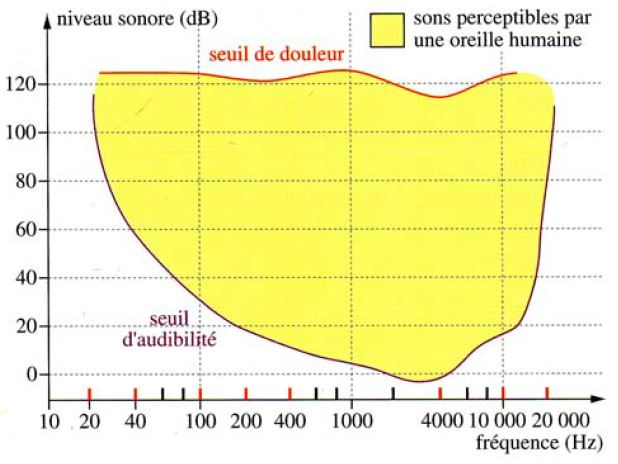
\includegraphics[width = \linewidth]{audition.jpg}
	\caption{Seuil de douleur et d'audibilité de l'oreille humaine}
\end{marginfigure}
